
\documentclass[12pt]{article}
 
\usepackage[margin=1in]{geometry} 
\usepackage{amsmath,amsthm,amssymb,scrextend}
\usepackage{fancyhdr}
\pagestyle{fancy}
\DeclareMathOperator{\rng}{Rng}
\DeclareMathOperator{\dom}{Dom}
\newcommand{\R}{\mathbb R}
\newcommand{\cont}{\subseteq}
\newcommand{\N}{\mathbb N}
\newcommand{\Z}{\mathbb Z}
\usepackage{tikz}
\usepackage{pgfplots}
\usepackage{amsmath}
\usepackage[mathscr]{euscript}
\let\euscr\mathscr \let\mathscr\relax% just so we can load this and rsfs
\usepackage[scr]{rsfso}
\usepackage{amsthm}
\usepackage{amssymb}
\usepackage{multicol}
%\usepackage{ngerman}
\usepackage[colorlinks=true, pdfstartview=FitV, linkcolor=blue,
citecolor=blue, urlcolor=blue]{hyperref}

\DeclareMathOperator{\arcsec}{arcsec}
\DeclareMathOperator{\arccot}{arccot}
\DeclareMathOperator{\arccsc}{arccsc}
\newcommand{\ddx}{\frac{d}{dx}}
\newcommand{\dfdx}{\frac{df}{dx}}
\newcommand{\ddxp}[1]{\frac{d}{dx}\left( #1 \right)}
\newcommand{\dydx}{\frac{dy}{dx}}
\let\ds\displaystyle
\newcommand{\intx}[1]{\int #1 \, dx}
\newcommand{\intt}[1]{\int #1 \, dt}
\newcommand{\defint}[3]{\int_{#1}^{#2} #3 \, dx}
\newcommand{\imp}{\Rightarrow}
\newcommand{\un}{\cup}
\newcommand{\inter}{\cap}
\newcommand{\ps}{\mathscr{P}}
\newcommand{\set}[1]{\left\{ #1 \right\}}
\newtheorem*{sol}{Solution}
\newtheorem*{claim}{Claim}
\newtheorem{problem}{Problem}
\begin{document}
 

\lhead{Formal Logic Sheet 7}
\chead{Robert Feldhans, Sebastian Mueller}
\rhead{\today}


\section*{Exercise 25:  (Drinker paradox)}

\section*{Exercise 26: (Barber paradox)}

\section*{Exercise 27: (Runtime)}

\section*{Exercise 28: (Find the box)}
Show that $\square \in Res(F)$\\
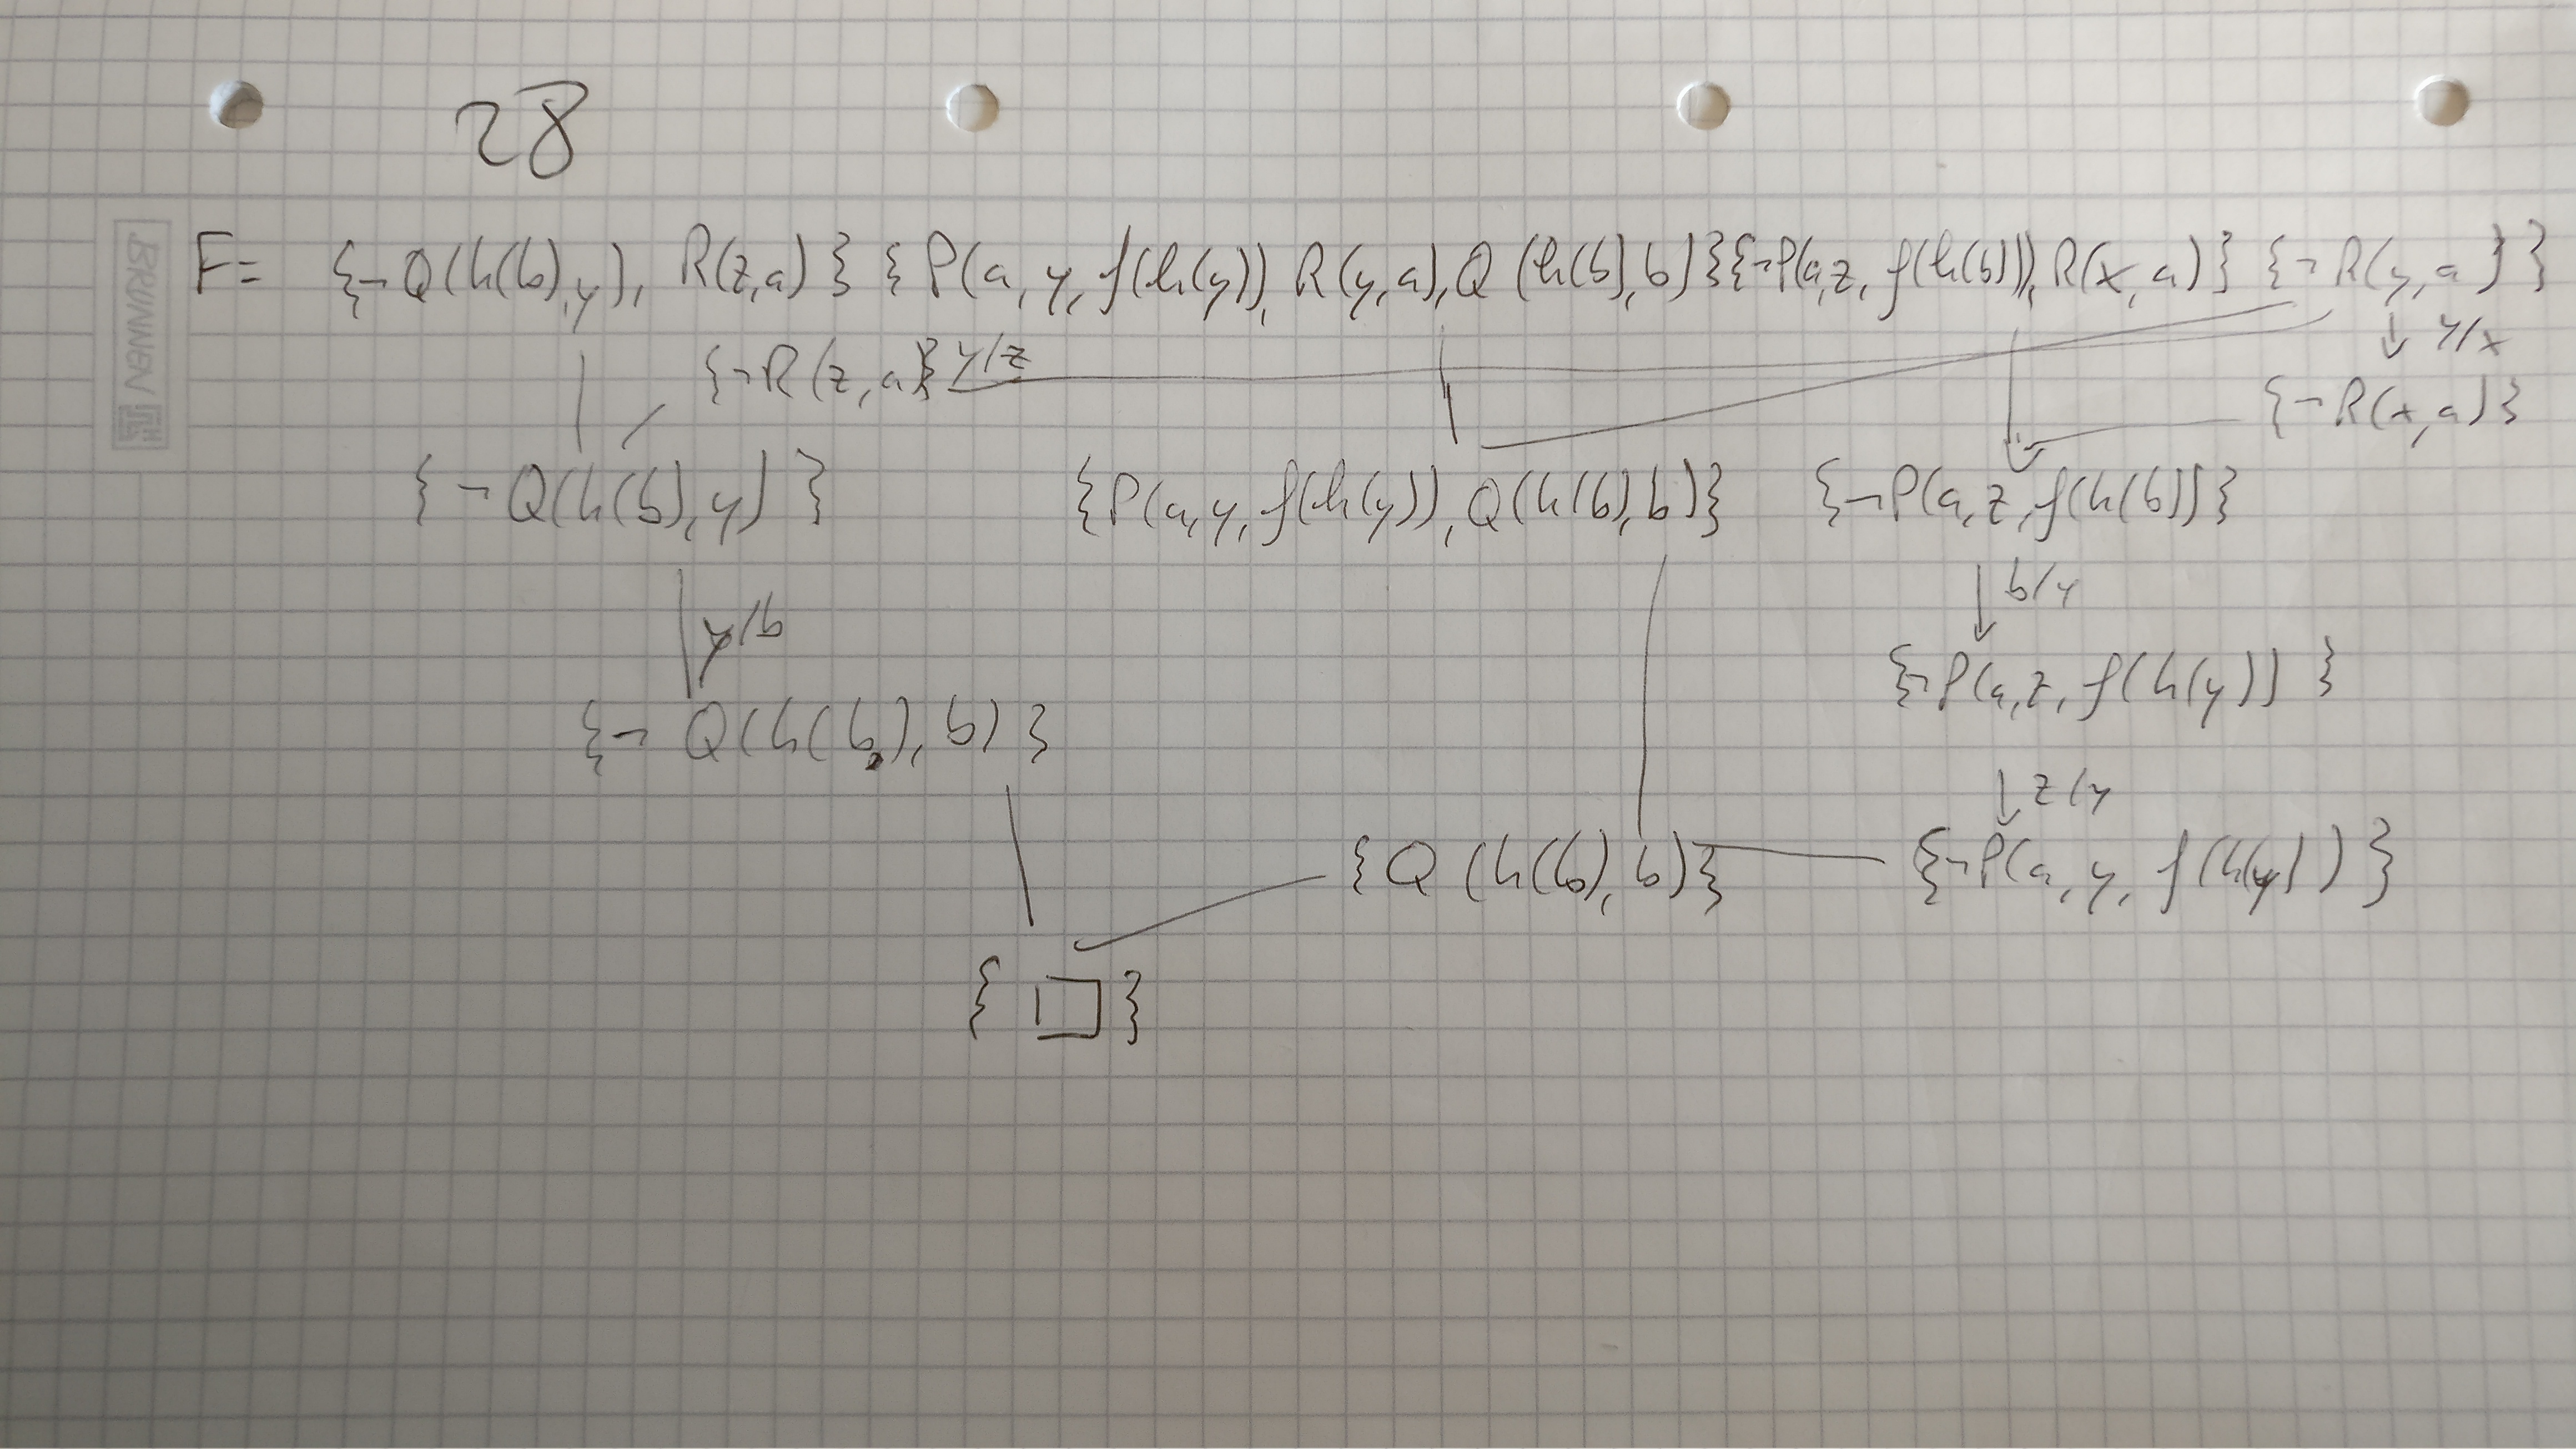
\includegraphics[width=\textwidth,height=\textheight,keepaspectratio]{./ex28.jpg}



%ANARCHY
\end{document}